\documentclass{article}
%\usepackage{msmath}
\usepackage{amssymb, amsmath}
\usepackage[pdftex]{graphicx}
\usepackage{listings}              % code insert
\usepackage{color}
\usepackage[usenames,dvipsnames,svgnames,table]{xcolor}
\usepackage{wrapfig}

\lstset{
    breaklines = true,
    numbers = left,
    stepnumber = 1,
    numberstyle=\color{black},
    showstringspaces=false,
    language=C,
    frame=rlTB,
    rulecolor= \color{blue},
    basicstyle=\scriptsize\ttfamily\color{red!80!black},
      keywordstyle=\bfseries\color{blue},
      commentstyle=\color{green!40!black},
      identifierstyle=\ttfamily\color{black},
      stringstyle=\color{yellow!65!black},
}

\newcommand{\ssection}[1]{
\addcontentsline{toc}{section}{#1}
\section*{#1}}


\title{G3 - report}
\author{Ask Neve Gamby \& Maya Saietz}

\begin{document}
\maketitle

\section{Thread-safe stack}
\subsection{The stack}
We have a struct type, \texttt{stack\_t}, which contains a pointer to the start of a singly linked list, and a mutex lock. The linked list contains void pointers as its elements, and is not thread-safe by itself -- only when used as the underlying structure for the stack.

The bottom element in the stack -- that is, the last element in the linked list -- has a \texttt{NULL}-pointer as the pointer to the next element. The empty stack has a \texttt{NULL}-pointer as the pointer to the linked list.

\paragraph{stack\_init}
The \texttt{top}-variable of the stack is set to \texttt{NULL} (the stack is empty), and the lock is initialized. We do not use any locking here, because (hopefully) no one has started modifying the stack yet.

\paragraph{stack\_empty} We first acquire the lock -- otherwise someone could pop or push to the stack while we're comparing things. We then compare the top of the stack to \texttt{NULL}, and store the result in a local variable. After releasing the lock, we can safely return the result of the comparison.

\paragraph{stack\_top}
This is slightly more complicated than \texttt{stack\_empty}. If the top of the stack is \texttt{NULL}, we immediately release the lock and return \texttt{NULL}. Otherwise, we return the contents of the top element (using the same technique of storing the result in a seperate variable, releasing the lock, and then returning).

\paragraph{stack\_pop}
This function is much like \texttt{stack\_top}. The big difference is that we have to change the \texttt{top}-pointer and free the previous top element. For this, we need a temporary variable where we can store the top element after changing the pointer, but before freeing it.

\paragraph{stack\_push}
This function creates a new linked list entry using \texttt{malloc}. If there is no space to allocate, we return 1. We set the entry's contents to the given pointer, and then we lock the stack. We put the new item on the stack, change the \texttt{top}-pointer and unlock the stack. Finally, we return 0.

\subsection{Matrix multiplication}
The code for representing a task and creating a row of the result matrix is taken more or less directly from demonstration program. The same thing goes for creating and printing the matrices, and handling arguments.

The \texttt{main} function first sets some variables based on the arguments, and then creates the three arrays. Two of them are initialized with random numbers. The result matrix is allocated with \texttt{calloc}, so it contains zeroes.

We then push all the tasks on our stack, and create the threads that will solve the tasks. Once we've started all the threads, we call \texttt{pthread\_join} on them (so we block until all threads are done). Finally, we call \texttt{free} on everything that we allocated with \texttt{malloc}.

Each thread runs the function \texttt{solve\_tasks}. This function keeps popping tasks from the stack and solving them one by one, until the stack is empty. When it is, the function returns \texttt{NULL}.

We don't lock either of the matrices. The two input matrices, \texttt{a} and \texttt{b}, are never modified once they've been initialized, and in the result matrix, each thread will only work on one row.

\subsubsection{Timing}
In order to measure how much we gain from using threads, we use \texttt{clock\_gettime}. We start measuring the time just before starting the threads, and we stop immediately after joining the last thread. We then gathered data for $10$ runs for each of a couple of settings (different amount of cores enabled on the virtual machine it is run on, and different amount of allowed threads). All runs where on calculating a random $800$ by $800$ matrix multiplication. We then calculate the mean, standard devition and standard deviation of mean. This data is composed into figure \ref{fig:stat}. Notice the drop from $1$ threads to pultiple threads. Looking at the data, it is likely that the virtual machine could not handle the hyperthreading, as the virtual machine program gave some warnings, and there is a significant increase in the time it took to run the program otherwise. One can see that there was not a very significant increase in the runtime after changing to $2$ or more threads, since much of the increased parallism is eaten up by overhead. This likely has to do with the speed being limmited by external factors like the syncronisation on the stack, while the actual matrix operations have been significantly limmited. We can also see that large amounts of threads still do help out a little bit compared to a number of threads just around the number of cores. This could be causes by the threads occupying a larger fraction of to total number of threads to be scheduled, and thereby get a larger fraction of the total alloted cpu time.

\begin{figure}
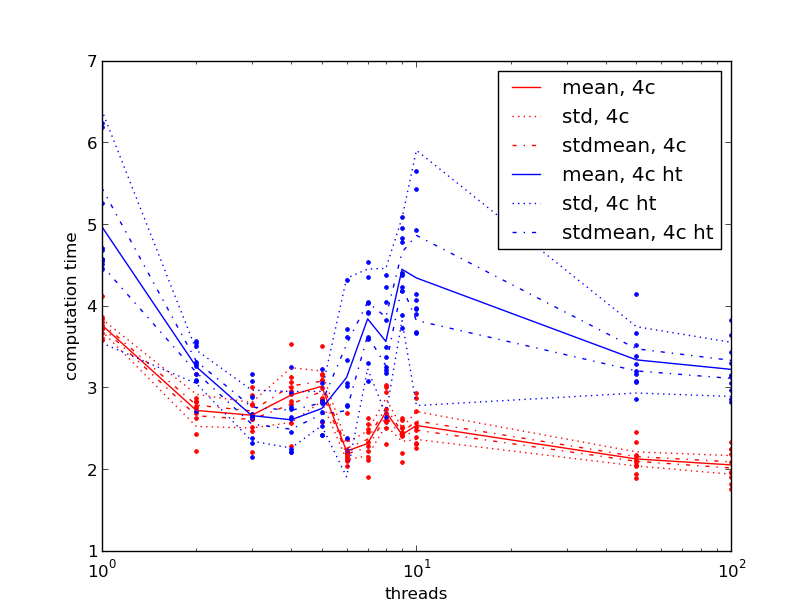
\includegraphics{figure_1.png}
\caption{A figure of some simple statistics of the matrix multiplcation program run with different number of threads, on either 4 cores (red) or 8 cores (blue) on a 4 cores with hyper treading macine running it in a virtual machine. Notice the seep drop $1$ and to the following, and how more threads than cores mostly gives more overhead. Also notice that the error on the mean is small enoug that we have no problems making conclusions.} 
\label{fig:stat}
\end{figure}

\section{Userland semaphores in Buenos}

Userland semaphores are implemented in \texttt{proc/semaphores.h} and \texttt{proc/semaphores.c}. The header file defines two types. \texttt{usr\_sem\_t} is \texttt{void}, and \texttt{usr\_sem\_entry} is a struct that contains a kernel semaphore, a name, and the number of threads that are blocked on that semaphore.

There are two important global variables -- \texttt{sem\_table} is a table of all user semaphores. \texttt{sem\_table\_lock} is a kernel semaphore which must be held while accessing \texttt{sem\_table}.

\paragraph{usr\_sem\_init}
This function does two things. It creates the global semaphore \texttt{sem\_table\_lock}, and it initializes every entry in \texttt{sem\_table} to have no kernel semaphore, and no stuck processes.

\paragraph{usr\_sem\_open}
This function has different behaviour depending on the second argument, \texttt{value}. If \texttt{value} is larger than or equal to zero, it tries to create a new semaphore. It does this by looking through the table and storing the first free position in a variable. It then goes through the rest of the table. If, at any point, it finds an already-active semaphore with the given name, it returns \texttt{NULL}.

Once we have the free entry, we copy over the name, create a new kernel semaphore, release the lock on the table and return.

If \texttt{value} is less than zero, we look through the table for a semaphore of the given name. If we find it, we return its handle. If not, we return \texttt{NULL}.

\paragraph{usr\_sem\_p}
This function is basically a glorified wrapper around the kernel-level \texttt{semaphore\_P}. It has some checks for whether the given handle is valid, and it locks the semaphore table while accessing it (making sure \emph{not} to hold it while calling \texttt{semaphore\_P}). It also modifies the counter of processes that are waiting on the semaphore.

\paragraph{usr\_sem\_v}
Much like \texttt{usr\_sem\_p}, this is a wrapper around \texttt{semaphore\_V} with some checks for whether the handle is valid. If it's not, we return a negative number.

\paragraph{usr\_sem\_destroy}
This function checks if there are any processes that are blocked on the semaphore. If there are, it returns -1. If not, it destroys the kernel-semaphore and sets the semaphore-pointer of the table entry to \texttt{NULL}, indicating that this user semaphore is free. It then returns 0.

The possible race condition is handled by acquiring \texttt{sem\_table\_lock} before checking if any processes are blocked.

For all the other funcions, the relevant \texttt{SYSCALL\_SEM\_*}-constant and wrapper function in \texttt{tests/lib.c} were already created, but for \texttt{syscall\_sem\_destroy}, we had to add them.

\subsection{Semaphore handles}
\texttt{usr\_sem\_t} is void, so the handle that the user program gets from \texttt{syscall\_sem\_open} is a void-pointer. However, we don't want it to be a pointer to anything useful -- userspace programs shouldn't modify or read kernel-space memory directly. Therefore, the pointer is created by taking the index into \texttt{sem\_table} and xor'ing it with \texttt{0xFFFFFFFF}. This gives us a pointer to something in userspace that we don't know what is.

We could have simply cast the index to a pointer and returned that, but this would make it easier for the user to do something stupid -- it would \emph{look} like an integer, and it could simply be incremented or decretmented to access the neighboring semaphores. Our solution isn't much better, but at least it \emph{pretends} to be a weird pointer to something useless. Another disadvantage to using the index is that index 0 would be indistinguishable from a \texttt{NULL}-pointer.

\subsection{Testing}
We have tested the user semaphores using the handed-out programs \texttt{barrier}, \texttt{prog0} and \texttt{prog1}. The programs run as expected -- one of them asks for input and echoes it back, then the other one, and only then are they allowed to finish.

\end{document}
